\section{Supplementary methods, controls and tables}
\label{app:supp}

This appendix holds the material that the argument does not need: the other DAX options, the detailed settings, the policy-log channel and its
control, run times, the algorithms, the checks of the pipeline, the search grids of the baselines, the closed-form controls, the sensitivity of the
Holm adjustment and the training seeds.

\subsection{Other DAX options}\label{app:fh}

The main experiment uses the switches described in Section~\ref{sec:method-dax}. The remaining values of the search grid are a prior strength of 160, a
lifelong strength of zero, the scenario factors switched off and no user groups. The main experiment did not select any of these in any split, so the user-group refinement is on in all five splits. The
ablation without a tag prior replaces the centre by one global mean. The grid tables in \ref{app:grids} give the chosen values.

\subsection{Detailed settings of LEAF, LEAF-LGN and DAX}\label{app:impl}

\paragraph{Temporal boundary} The cut-off $T_0$ is 22 April 2022, 00:00 (UTC+8), the start of the random-exposure period. The latest impression used for
training precedes $T_0$ by about two seconds, and the earliest random impression used for evaluation follows it by about ten hours. The lifelong
statistics, the DAX fit, the popularity offset and the negative sampler read only events before $T_0$.

\paragraph{LEAF statistics} The shrinkage strength of the lift in Equation~\eqref{eq:lift} is $\eta=5$ pseudo-impressions. On KuaiRand-27K, 26,904 users
have a lifelong history before $T_0$, and 44 tag values, 6,510 author values and 7,202 music values occur on pool videos. A missing key value, or a value
that the user never saw, gives a channel of exactly zero.

\paragraph{LEAF-LGN} The embedding dimension is $d=64$. The scoring embeddings mix the layer-zero embedding and the two propagated layers. The biases
$b_u$, $b_i$ and $b_0$, the popularity weight $\beta$ and the channel weights $g$ are initialised at zero, and weight decay applies to the embeddings only.
Training uses Adam with batches of 8,192 triples and at most 40 epochs. For each split, training stops after three epochs without an improvement of the
best validation nDCG@10. A negative item that falls in the excluded set is redrawn once. The search covers the learning rate, the weight decay and the
policy weight $w\in\{0,0.25,0.5\}$, which gives twelve trainings (\ref{app:grids}).

\paragraph{DAX} The factors start at $\theta_u=0.7$, $\kappa_t=1$ and $\alpha_i=0.6$, and the EM runs for 40 iterations without a convergence test
(\ref{app:em} gives the clamps). The scenario factors are relative to the evaluation scenario and may exceed one. Without the scenario factor,
$\kappa_t=1$ for all $t$. The median number of policy-log impressions per pool item is 43. Of the pool items, 0.6\% have none and receive the centre of
their tag.

\paragraph{Combination} The weight $\gamma$ takes the ten values of \ref{app:grids}. The early-stopping rule of a split uses the best validation
value over all candidates of an epoch, the backbone and the combined scores alike.

\subsection{Policy-log channel}\label{app:policy}

For a pair $(u,i)$ let $N_{ui}=1$ if $u$ was shown $i$ before $T_0$ and never clicked it. The policy-log channel adds these shown but unclicked pairs to the
BPR loss of Equation~\eqref{eq:bpr} as positives. In each epoch each such pair is used as a positive with probability $w\in[0,1]$, which sets how much the
decision to show the item counts as weak evidence of relevance. Negatives are drawn uniformly from the items that $u$ was not shown before $T_0$ when
$w>0$, and from the items that $u$ did not click when $w=0$.

The selected weight differs between the models. The separately tuned LEAF-LGN selects $w=0$ in the first four splits and $w=0.25$ in the fifth. The
LEAF-LGN of the main table selects $w=0$ in all five splits. The LEAF-LGN+DAX backbone selects $w=0.25$ in the first and fourth splits and $w=0.5$
in the other three. In the separately tuned model, removing the channel gives identical test scores in four splits and, in the fifth, a score higher by
$2.4\times10^{-3}$ (Table~\ref{tab:policy}). The control was not run on LEAF-LGN+DAX.

\begin{table}[tbp]
\centering
\footnotesize
\caption{Policy-channel control on KuaiRand-27K: the separately tuned LEAF-LGN with and without the policy-log channel (nDCG@10). Selected weight: zero in four of the five splits.}
\label{tab:policy}
\begin{adjustbox}{max width=\linewidth}
\begin{tabular}{lrrrrrr}
\toprule
Variant & Configurations & Mean & Difference [95\% hw] & Per-user $p$ & NB $p$ & NB $p_{\mathrm{Holm}}$ \\
\midrule
LEAF-LGN (separate search, reference) & 197 & 0.4728 & n/a & n/a & n/a & n/a \\
\midrule
without policy channel & 4 & 0.4733 & -0.55 [0.33] & $1.13\times10^{-3}$ & 0.793 & 0.793 \\
\bottomrule
\end{tabular}
\end{adjustbox}
\par\smallskip
\begin{minipage}{\linewidth}\raggedright\footnotesize Difference: the reference minus the variant, so a positive value means that the removed signal helps. The variant is selected on validation users over its own grid of 4 configurations, and the reference over 197 configurations, which favours the reference. Per-user $p$: two-sided paired t test over the pooled test users. NB $p$: Nadeau-Bengio test over the five split means. NB $p_{\mathrm{Holm}}$: Holm adjustment over the three controls of Table~\ref{tab:leafctl-lgn} and this one.\end{minipage}
\end{table}


\subsection{Run times}\label{app:cost}

The LEAF tables are dense user-by-key arrays for the three key families, with one row per user. A pair is a gather, which costs a constant amount per
pair, and the tables are built in one streaming pass over the lifelong log. The LightGCN propagation costs $O(L|E|d)$ per epoch, where $|E|$ is the number
of clicked pairs, and each sampled pair adds a constant amount for the channels. Each DAX iteration is linear in the number of pre-cut impressions plus
the numbers of users, items and scenarios. The main search fitted 32 DAX tables in 1.8 to 3.3 seconds each, and trained the twelve LEAF-LGN backbones in 884
to 2,437 seconds each, with a total wall time of about 19,600 seconds on two CPU threads.

\subsection{Algorithms}
\label{sec:method-algorithms}

Algorithm~\ref{alg:dax} gives the DAX fit, and Algorithm~\ref{alg:leaflgn} gives the training and selection of LEAF-LGN+DAX.

\begin{algorithm}[t]
\caption{DAX-EM on the pre-cut log}
\label{alg:dax}
\begin{algorithmic}[1]
\Require pre-cut impressions $(u_r,i_r,t_r,y_r)$, tag groups, lifelong rates $r_u$, prior strengths $\nu,\lambda$, 40 iterations
\State $\theta_u\gets 0.7$, $\kappa_t\gets 1$, $\alpha_i\gets 0.6$
\For{$it=1,\dots,40$}
  \For{each impression $r$} \Comment{E-step}
    \If{$y_r=1$}\ $p_{E,r}\gets 1$, $p_{R,r}\gets 1$
    \Else\ $\tau_r\gets\theta_{u_r}\kappa_{t_r}$, $p_{E,r}\gets\tau_r(1-\alpha_{i_r})/(1-\tau_r\alpha_{i_r})$,
      $p_{R,r}\gets(1-\tau_r)\alpha_{i_r}/(1-\tau_r\alpha_{i_r})$
    \EndIf
  \EndFor
  \State $\tilde c_u\gets\mathrm{clip}_{[10^{-3},1]}\bigl(\tfrac{r_u}{\bar r}\sum_r p_{E,r}/\sum_r\kappa_{t_r}\bigr)$ \Comment{lifelong centre}
  \State $\theta_u\gets(\sum_{r:u_r=u}p_{E,r}+\lambda\tilde c_u)/(\sum_{r:u_r=u}\kappa_{t_r}+\lambda)$, clipped
  \State $\kappa_t\gets(\sum_{r:t_r=t}p_{E,r}+1)/(\sum_{r:t_r=t}\theta_{u_r}+1)$; \ $\kappa\gets\kappa/\kappa_1$
  \State $c_g\gets(\sum_{i\in g}\sum_{r:i_r=i}p_{R,r}+1)/(\sum_{i\in g}n_i+2)$ for each tag group $g$, \ $c_i\gets c_{\mathrm{tag}(i)}$
  \State $\alpha_i\gets(\sum_{r:i_r=i}p_{R,r}+\nu c_i)/(n_i+\nu)$, clipped
\EndFor
\State \Return $\operatorname{logit}\alpha$, $\theta$, $\kappa$
\end{algorithmic}
\end{algorithm}

\begin{algorithm}[t]
\caption{Training and selection of LEAF-LGN+DAX}
\label{alg:leaflgn}
\begin{algorithmic}[1]
\Require pre-cut log, the twelve backbone settings $(\mathrm{lr},\rho,w)$, the 32 DAX configurations, the ten values of $\gamma$, five splits of the validation and test users
\For{each backbone setting $(\mathrm{lr},\rho,w)$}
  \State train LEAF-LGN (BPR, policy weight $w$) one epoch at a time, at most 40 epochs
  \State fit DAX once per configuration (Algorithm~\ref{alg:dax}), giving $\operatorname{logit}\alpha$
  \For{each epoch}
    \State compute $s^{\mathrm{LEAF}}_{ui}$ on the candidates of every validation and test user
    \For{each DAX configuration and each $\gamma$}
      \State $s_{ui}\gets\operatorname{std}_{C_u}(s^{\mathrm{LEAF}}_{ui})+\gamma\operatorname{std}_{C_u}(\zeta_i)$ \Comment{$\gamma=0$ is the backbone}
      \For{each split $s$ still active}
        \If{validation nDCG@10 of $s_{ui}$ exceeds the best value of $s$}
          \State record the configuration, the epoch, $\gamma$, and the test nDCG@10 of $s$
        \EndIf
      \EndFor
    \EndFor
    \State each split stops after three epochs without a gain in its best validation value
  \EndFor
\EndFor
\State \Return for each split the recorded configuration with the best validation value and its test value
\end{algorithmic}
\end{algorithm}

\subsection{Checks of the pipeline and reproducibility}\label{app:controls}

The temporal boundary was checked by construction and by test. No training input postdates $T_0$. The random-exposure labels enter only the scores:
changing the labels of the validation and test users changes the reported nDCG@10 and nothing else. The lifelong tables and the DAX parameters do not change
when rows from after the cut-off, or from the pool, are altered. The sequence models see only events before the cut-off that are not pool videos. The user
identifiers of the two releases agree for 99.99\% of the joined events, and the counts of out-of-pool impressions differ by less than 0.02\% between the raw
logs and the pooled tables.

On simulated data with known parameters, the lift and familiarity statistics reproduce their definitions, and the lifelong gain of a synthetic user population
falls below 0.03 in absolute value when the users' tables are shuffled. With negligible priors the observed-data likelihood of the DAX fit does not decrease over the first 25
iterations, for three starting seeds. The recovered attractiveness has a Spearman correlation above 0.8 with the true attractiveness, and the recovered
examination propensity has one above 0.75 with the true propensity. The additive variant recovers item appeal with a correlation above 0.5. Within-tag
permutation keeps less than 30\% of a synthetic gain, and the across-item permutation is a bijection of the items.

Table~\ref{tab:controls-real} gives the preliminary controls on real data. They are computed on fixed backbone scores, and the values are diagnostic rather than
the main results. All tables of the paper are generated from the recorded per-split results by one analysis, and each number in the text is copied from its output.

\begin{table}[tbp]
\centering
\caption{Preliminary controls on the real data, on fixed backbone scores unless stated otherwise. Differences are in units of $10^{-3}$ nDCG@10, with the 95\% half-width in brackets.}
\label{tab:controls-real}
\footnotesize
\renewcommand{\arraystretch}{1.1}
\begin{tabular}{p{0.44\textwidth}p{0.48\textwidth}}
\toprule
Control & Result \\
\midrule
Users' lifelong tables shuffled, closed-form scorer & Full minus shuffled: $+18.90$ [1.99]; the shuffled variant and the variant without lifelong channels differ by $-1.02$ \\
Users' lifelong tables shuffled, LEAF-LGN & The lifelong channels on shuffled tables give $-0.93$ [0.45] \\
Attractiveness permuted across items & Gain $-0.27$ [0.36]: the gain is removed \\
Attractiveness permuted within tags & Gain $+6.28$ [1.10], that is 41.6\% of the full gain \\
Tag mean alone; within-tag permutation; full DAX & $+4.31$ [1.07]; $+3.29$ [0.99]; $+9.45$ [1.36] \\
Permutation across items, selected policy weight & The selected policy weight is zero in all five splits in this analysis \\
Full DAX in the ablation search & The same configurations are selected in all five splits, with the same test values \\
LEAF-LGN reproduction & Main-search LEAF-LGN minus separately tuned LEAF-LGN: $+0.73$ [0.52], Nadeau-Bengio $p=0.660$ \\
Off-protocol calibration & Adding the validation users' random-exposure rate to LEAF-LGN: $+36.62$ [1.79]. This uses post-cut labels and is a diagnostic, not a method \\
\bottomrule
\end{tabular}
\end{table}

\subsection{Baselines and search grids}\label{app:baselines}

All baselines are trained on the same pre-cut log with the same splits and the same selection rule, and Table~\ref{tab:baselines} lists their grids. Every backbone with DAX gets the same DAX module and the
same $\gamma$ grid as LEAF-LGN.

\begin{table}[t]
\centering
\caption{Baselines, search grids and configurations searched. SIM denotes SIM-hard; $\rho$ is the weight decay and $d$ the embedding dimension.}
\label{tab:baselines}
\footnotesize
\begin{adjustbox}{max width=\textwidth}
\begin{tabular}{p{0.22\textwidth}p{0.62\textwidth}r}
\toprule
Method & Search grid & Configurations \\
\midrule
\raggedright LightGCN \citep{he2020lightgcn} & \raggedright learning rate $\{10^{-2},3\cdot10^{-3}\}$, $\rho\in\{10^{-5},10^{-4}\}$; $d=64$, 2 layers, at most 40 epochs, patience 3 & 4 \\
\raggedright r-AdjNorm \citep{zhao2022radjnorm} & \raggedright LightGCN grid with normalisation exponent $r\in\{0.3,0.7\}$ & 8 \\
\raggedright PW-LightGCN (\ref{app:qp}) & \raggedright DR-BPR-LGN-1, -p2 and -p with their own grids; per split the best of the three & 20 \\
\raggedright PW-LightGCN + DAX & \raggedright the 10 distinct (method, configuration) trainings chosen by any split of the PW-LightGCN search, with the DAX grid & 3,200 \\
\raggedright EASE \citep{steck2019ease} & \raggedright closed form, $\lambda_{\mathrm{EASE}}\in\{1000,3000,10000\}$, $w\in\{0,0.25,0.5\}$, popularity weight $\beta\in\{0,0.25,0.5\}$ & 27 \\
\raggedright EASE + DAX & \raggedright EASE with the DAX grid & 8,640 \\
\raggedright LEAF-LGN & \raggedright 12 trainings (learning rate, $\rho$, $w$), no DAX & 12 \\
\raggedright LEAF-LGN + DAX & \raggedright 12 trainings with the DAX grid and $\gamma$ & 3,840 \\
\raggedright DIN (deep interest network; \citealp{zhou2018din}) & \raggedright 4 trainings (learning rate, $\rho$); dimension 16, hidden 16, MLP 32, batch 1024, at most 12 epochs, patience 2; last $L=200$ pre-cut events & 4 \\
\raggedright DIN + DAX & \raggedright 4 trainings with the DAX grid and $\gamma$ & 1,280 \\
\raggedright SIM-hard \citep{pi2020sim} & \raggedright as DIN, with the $K=50$ most recent events sharing the tag or author of the candidate & 4 \\
\raggedright SIM-hard + DAX & \raggedright as DIN + DAX & 1,280 \\
\raggedright NAVIP \citep{kim2022navip} & \raggedright propensity-weighted graph model with two propagation layers; learning rate $\{10^{-2},3\cdot10^{-3}\}$, $\rho\in\{10^{-5},10^{-4}\}$; $d=64$, at most 40 epochs, patience 3; propensity from item popularity & 4 \\
\raggedright IPS-MF \citep{schnabel2016} & \raggedright matrix factorisation with inverse-propensity weights; the same grid and propensity & 4 \\
\raggedright DR-JL \citep{wang2019drjl} & \raggedright doubly robust joint learning; the same grid and propensity & 4 \\
\raggedright MRDR \citep{guo2021mrdr} & \raggedright doubly robust matrix factorisation estimator; the same grid and propensity & 4 \\
\raggedright Closed-form LEAF scorer (no graph training; controls only) & \raggedright closed-form grid over the ridge penalty, the policy weight and the channel weights & 3,456 \\
\raggedright LightGCN + DAX & \raggedright the DAX grid and $\gamma$ on the same-run LightGCN base (3 trainings) & 960 \\
\bottomrule
\end{tabular}
\end{adjustbox}
\end{table}

\subsection{Closed-form LEAF scorer controls}\label{app:leafctl}

These controls use a closed-form LEAF scorer, with the same six channels and no graph training, (Table~\ref{tab:leafctl}). They are secondary to the
controls on LEAF-LGN of Section~\ref{sec:res-controls}. Shuffling the users' lifelong tables across users gives the largest loss, $+18.90$ [1.99] (Holm
adjusted over the eight arms $4.90\times10^{-76}$; Nadeau-Bengio adjusted $4.60\times10^{-3}$), and removing all lifelong channels gives $+17.88$ [2.04]. The
policy channel contributes $+5.01$ [1.20] per user, but its split-level value is not significant after Holm adjustment (Nadeau-Bengio adjusted 0.132). The
variant without music channels gives identical rankings.

\begin{table}[tbp]
\centering
\footnotesize
\caption{LEAF controls on KuaiRand-27K, secondary: closed-form LEAF-tied backbone, variant means and full minus variant.}
\label{tab:leafctl}
\begin{adjustbox}{max width=\linewidth}
\begin{tabular}{lrccccc}
\toprule
Variant & Configs & Mean & Full minus variant [95\% hw] & $p_{\mathrm{Holm}}$ & NB $p$ & NB $p_{\mathrm{Holm}}$ \\
\midrule
LEAF-tied (full) & 3456 & 0.4691 & n/a & n/a & n/a & n/a \\
\midrule
users' lifelong statistics shuffled & 3456 & 0.4499 & +18.90 [1.99] & $4.90\times10^{-76}$ & 0.001 & $4.60\times10^{-3}$ \\
without tag channels & 1152 & 0.4594 & +9.38 [1.63] & $1.17\times10^{-28}$ & 0.002 & $6.48\times10^{-3}$ \\
without author channels & 432 & 0.4628 & +6.45 [1.17] & $2.10\times10^{-26}$ & 0.001 & $4.42\times10^{-3}$ \\
without lifelong channels & 72 & 0.4512 & +17.88 [2.04] & $9.61\times10^{-65}$ & 0.000 & $2.51\times10^{-3}$ \\
without policy channel & 864 & 0.4643 & +5.01 [1.20] & $6.91\times10^{-16}$ & 0.066 & $1.32\times10^{-1}$ \\
lift only & 432 & 0.4634 & +5.78 [1.11] & $6.10\times10^{-24}$ & 0.001 & $4.60\times10^{-3}$ \\
familiarity only & 576 & 0.4585 & +10.26 [1.66] & $4.07\times10^{-33}$ & 0.001 & $4.60\times10^{-3}$ \\
without music channels & 1728 & 0.4691 & 0.00 [0.00] & 1 & 1.000 & 1 \\
\bottomrule
\end{tabular}
\end{adjustbox}
\par\smallskip
\begin{minipage}{\linewidth}\raggedright\footnotesize Full minus variant: positive means the channel helps. Holm within the eight variants; NB over the split means. The variant without music channels gives identical rankings in every split. These controls were run on the closed-form LEAF-tied backbone.\end{minipage}
\end{table}


\subsection{Sensitivity of the Holm adjustment}\label{app:sens}

Table~\ref{tab:sens} extends the main family of thirteen by EASE and EASE+DAX, giving a family of fifteen. The per-user p values are given in the same table.
The conclusions at the 0.05 level are unchanged, and the two split-level values closest to the threshold stay at $4.56\times10^{-2}$.

\begin{table}[tbp]
\centering
\footnotesize
\caption{Sensitivity of the Holm adjustment: the main family extended by EASE and EASE+DAX, with per-user and split-level values (the family size is given in the column header).}
\label{tab:sens}
\begin{adjustbox}{max width=\linewidth}
\begin{tabular}{lrccc}
\toprule
Comparator & Per-user $p$ & Per-user $p_{\mathrm{Holm}}$ (family of $11$) & NB $p$ & NB $p_{\mathrm{Holm}}$ \\
\midrule
QP family & $3.64\times10^{-125}$ & $2.91\times10^{-124}$ & 0.023 & $4.56\times10^{-2}$ \\
QP family+DAX & $3.96\times10^{-47}$ & $7.92\times10^{-47}$ & 0.006 & $2.23\times10^{-2}$ \\
LEAF-LGN & $6.55\times10^{-57}$ & $1.97\times10^{-56}$ & 0.001 & $6.85\times10^{-3}$ \\
r-AdjNorm & $2.43\times10^{-123}$ & $1.70\times10^{-122}$ & 0.000 & $3.91\times10^{-4}$ \\
LightGCN & $5.33\times10^{-190}$ & $5.33\times10^{-189}$ & 0.008 & $2.44\times10^{-2}$ \\
DIN & $1.41\times10^{-73}$ & $7.03\times10^{-73}$ & 0.001 & $6.62\times10^{-3}$ \\
DIN+DAX & $7.95\times10^{-12}$ & $7.95\times10^{-12}$ & 0.043 & $4.56\times10^{-2}$ \\
SIM & $3.55\times10^{-144}$ & $3.20\times10^{-143}$ & 0.000 & $3.14\times10^{-4}$ \\
SIM+DAX & $1.39\times10^{-59}$ & $5.56\times10^{-59}$ & 0.001 & $6.13\times10^{-3}$ \\
EASE & $6.53\times10^{-205}$ & $7.19\times10^{-204}$ & 0.000 & $1.31\times10^{-3}$ \\
EASE+DAX & $1.52\times10^{-115}$ & $9.13\times10^{-115}$ & 0.001 & $6.13\times10^{-3}$ \\
\bottomrule
\end{tabular}
\end{adjustbox}
\par\smallskip
\begin{minipage}{\linewidth}\raggedright\footnotesize The Holm values differ from Table~\ref{tab:main} only through the family size. Per-user p values are paired t tests over the pooled test users.\end{minipage}
\end{table}


\subsection{Training seeds}\label{app:seeds}

Training seeds 1 to 3 for LEAF-LGN+DAX, with the reduced search described in Section~\ref{sec:res-seeds}. Table~\ref{tab:seeds} and Figure~\ref{fig:seeds} give the seeds.

\begin{table}[tbp]
\centering
\footnotesize
\caption{Training seeds on KuaiRand-27K: LEAF-LGN+DAX and its within-seed gain over LEAF-LGN, for seeds 0 to 3.}
\label{tab:seeds}
\begin{adjustbox}{max width=\linewidth}
\begin{tabular}{lrrrccc}
\toprule
Seed & LEAF-LGN+DAX & LEAF-LGN & Configs & Gain [95\% hw] & $p$ & NB $p$ \\
\midrule
0 (main experiment) & 0.4854 & 0.4736 & 3840 & +11.96 [1.47] & $6.55\times10^{-57}$ & 0.001 \\
1 & 0.4858 & 0.4714 & 640 & +14.67 [1.42] & $1.63\times10^{-90}$ & 0.001 \\
2 & 0.4856 & 0.4708 & 640 & +15.10 [1.46] & $1.87\times10^{-90}$ & 0.002 \\
3 & 0.4844 & 0.4716 & 640 & +12.89 [1.44] & $1.90\times10^{-68}$ & 0.002 \\
\midrule
Spread over seeds & 0.4853 $\pm$ 0.0006 &  &  & +13.65 $\pm$ 1.48 &  &  \\
\bottomrule
\end{tabular}
\end{adjustbox}
\par\smallskip
\begin{minipage}{\linewidth}\raggedright\footnotesize Seed 0 is the main experiment with the full backbone search (12 trainings). Seeds 1 to 3 re-train with the training seed changed and a reduced backbone search: $\mathrm{lr}=3\times10^{-3}$ and $\rho=10^{-4}$ in every split, $w\in\{0.25,0.5\}$ for the DAX variant (two trainings) and $w=0.25$ for the base. The epoch, the DAX configuration and $\gamma$ are selected on validation in each split. Raw p values, not Holm-adjusted. The QP family was not re-trained under seeds 1 to 3, so no seed comparison with it is reported.\end{minipage}
\end{table}


\begin{figure}[tbp]
\centering
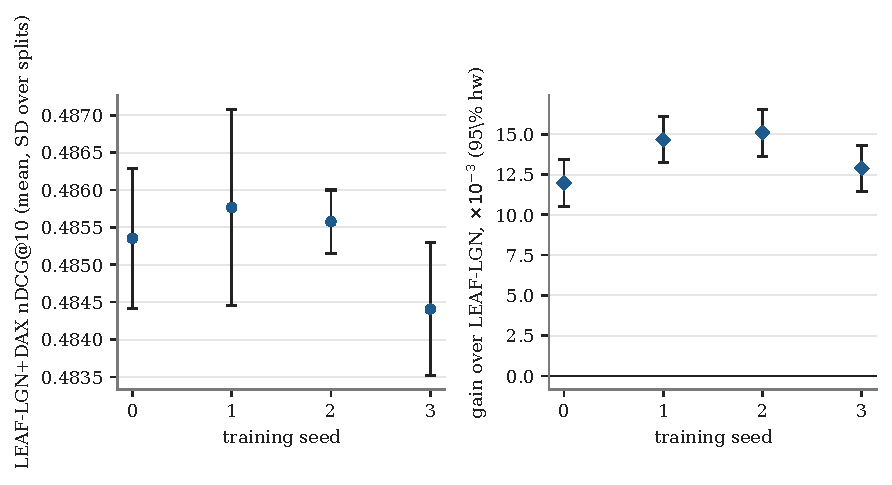
\includegraphics[width=0.85\linewidth]{figs/fig_seeds.pdf}
\caption{Training seeds 0 to 3 on KuaiRand-27K. Left: LEAF-LGN+DAX mean nDCG@10 with the standard deviation over splits, on an axis from 0.45 to 0.50. Right:
within-seed gain over LEAF-LGN, in units of $10^{-3}$, with the 95\% half-width.}
\label{fig:seeds}
\end{figure}
